\chapter{基于样本的快速图像填充}
\label{cha:Inpainting}
本章针对图像填充问题进行了研究,提出了一种基于样本的快速图像填充算法。为了使填充后的图像保持图像原有的结构信息,该算法以由粗到精的方式对图像中的缺失部分进行两次填充。在第一次填充时,首先利用离散小波变换(DWT)对输入图像进行预处理。利用DWT的特点,提取低频子带下的低分辨率图像。利用基于样本的填充方法在此低分辨率图像上进行填充。由于低分辨率图像中的高频细节部分已经被去掉,因此第一遍填充的图像的纹理和大部分结构信息都恢复得不错,但是在包含边界的局部区域还存在着一些瑕疵。为了解决这一问题,对原图像进行第二次填充,在这次填充时只处理包含边缘结构信息的部分,使得这部分区域的结构信息能够与图像的其他部分保持连续性。为了提高图像填充的速度,提出了以动态搜索窗口结合分块结构测试的方式来搜索最佳匹配块。实验结果证明,本章所提的算法能够处理各种困难情况,达到了与目前最好的算法相近的效果。但是,本章所提的算法速度明显优于这些算法。
\section{研究背景}
\label{background}
图像填充问题的主要困难在于使得图像中填充后的区域在内容和结构上与周围区域保持连续性以及算法的效率。相比而言,基于样本的算法在处理结构连续性方面更好。基于样本的算法的出发点是图像中缺失部分的像素,可以以分块为单位,利用图像中已知区域中的一个或多个最佳匹配分块来填充。Criminisi等人~\cite{Criminisi04regionfilling}提出了一种基于未知区域边界法线辐射度方向计算填充优先级算法,使得未知区域以一种类似``剥洋葱皮''的顺序进行填充。虽然该算法在一些缺失部分以纹理区域为主的图像中取得了不错的效果,但是对于缺失部分包含明显图像边缘等结构信息的情况却效果不佳。如图~\ref{fig:criminisi}所示,图~\ref{fig:criminisi:1}是待处理图像,其中黑色区域为缺失部分,图~\ref{fig:criminisi:2}为文献~\inlinecite{Criminisi04regionfilling}中算法的处理结果。可以看出,填充后的三角形金字塔尖并没有恢复,填充结果存在明显的不连续情况。Xu等人~\cite{Xu:2010}指出 为了保持结构部分的连续性,应该优先填充那些包含结构信息的分块。对于图~\ref{fig:criminisi:1}中的未知区域,金字塔部分具有明显的边缘结构信息,而天空部分则为平坦的纹理区域。如果在填充时优先填充金字塔部分然后在填充天空部分,则可以避免用包含金字塔部分的分块去填充天空部分。\par
\begin{figure}[htb]
  \centering%
  \subcaptionbox{输入图像\label{fig:criminisi:1}} %标题的长度,超过则会换行,如下一个小图。
    {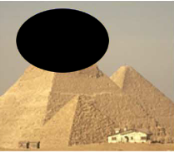
\includegraphics[width=0.3\textwidth]{fillM.png}}%
 \hspace{1em}%
  \subcaptionbox{文献~\inlinecite{Criminisi04regionfilling}算法填充结果\label{fig:criminisi:2}}
      {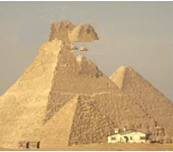
\includegraphics[width=0.3\textwidth]{fillMC.png}}
  \caption{文献~\inlinecite{Criminisi04regionfilling}算法失败例子}
  \label{fig:criminisi}
\end{figure}
在基于样本的图像填充算法中,由于像SSD这样的分块相似性度量指标的计算复杂度为$O(N_2)$,且搜索空间为图像全部已知区域,寻找每个缺失部分分块的最佳匹配块是一项非常耗时的工作。对于中等大小的图像,一些算法~\cite{Xu:2010}需要几分钟的时间来处理,这其中大部分时间用于分块的比较和搜索上。在实时或在线图像编辑等实际应用中,用户一般无法忍受超过1分钟的处理时间。\par
针对以上两方面的问题,本章提出利用基于梯度结构张量(gradient structure tensor,GST)来确定填充顺序,保持填充后图像的结构连续性。为了提高算法速度,提出了一种高效的分块结构测试方法对分块进行结构相似性度量,当分块间的结构信息存在较大差距时可以直接判为不匹配分块,减少冗余的SSD计算。同时,为了减少最佳匹配块的搜索范围,提出了一种动态搜索窗口算法,利用图像的连续性减少搜索范围。在分块匹配时,提出了用加权SSD代替SSD进行,以改进分块间的匹配度。

\section{算法描述}
\label{algorithm}
设输入图像\emph{I} 中包含未知区域 \(\Omega\) 已经已知区域 \(\overline{\Omega}\),本章提出的基于样本的图像填充算法的目标是通过\(\overline{\Omega}\)的信息来计算 \(\Omega\)。和其他经典的基于样本的填充算法那一样,本章所提算法的主要任务是确定填充优先级以及寻找最佳匹配块。
\subsection{基于GST的填充优先级}
\label{sec:sub:GST}

定义未知区域\(\Omega\) 的轮廓为 \(\partial\Omega\), 对于 \(\partial\Omega\)上的每个像素\(p\),将以\(p\)为中心的分块\(\Psi_p\)的填充优先级定义为:
\begin{equation}
   \label{equ:chap3:order}
   P(p)=C(p)\times D(p)
\end{equation}

其中 \(C(p)\) 表示可靠性项\cite{Criminisi04regionfilling},具体定义为: $$C(p)=\frac{\sum_{q\in\Psi_p\bigcap\overline{\Omega}}{C(q)}}{\left\vert{\Psi_p}\right\vert},其中$$\(\left\vert.\right\vert\)  表示计算分块中的像素数. 引入\(C(p)\) 的目的在于让那些包含更多已知像素的区域获得更高的优先级。~\ref{equ:chap3:order}中\(D(p)\) 是数据项,主要评估分块中包含结构信息的情况,增加那些包含较多结构信息分块的填充优先级。Xu等人\cite{Xu:2010}和Lemeur等人\cite{LeMeur_2011}分别提出了不同的\(D(p)\)计算方法。本章中提出了一种基于GST的方法。由于GST可以很好的描述图像的结构信息以及梯度方向,已经被广泛运用于图像处理领域\cite{Kothe03edgeand}。 \par
 对于图像\(I\), 其GST定义为:
 $$T=\left(\begin{array}{cc}T_{11} & T_{12} \\ T_{21} &T_{22}\end{array}\right)=\left(\begin{array}{cc}\overline{I_{\sigma,x}^2} & \overline{I_{\sigma,x}I_{\sigma,y}} \\ \overline{I_{\sigma,x}I_{\sigma,y}} & \overline{I_{\sigma,y}^2}\end{array}\right),$$ 
 其中 \(I_{\sigma,x}\) and \(I_{\sigma,y}\)  为图像在水平方向和垂直方向上的梯度 ,\(\overline{X}\) 表示高斯核函数\(G_{\hat{\sigma}}\) 与 \(X\)的卷积. \(T\) 的特征值 \(\lambda_1\) 和 \(\lambda_2\) 可以反映图像所包含的结构信息情况。在包含较强边缘信息的区域有 \(\lambda_1>\lambda_2\approx0\) ,而在不含边缘的平坦区域则有\(\lambda_1\approx\lambda_2\approx0\)。 \( \lambda_{1,2} \) 可以通过下式计算: $$\lambda_{1,2}=\frac{1}{2}\left(T_{11}+T_{22}\pm\sqrt{\left(T_{11}-T_{22}\right)^2+4T^2_{12}}\right)$$ 
 所包含结构的方向信息可以通过下式计算:
$$\phi=\frac{1}{2}\arctan{\left(\frac{2T_{12}}{T_{11}-T_{22}}\right)}$$

\section{实验结果与分析}
\label{results}


\section{本章小结}
\label{conclusions}




